\chapter{Feedback del CSI a tasso variabile}

\thispagestyle{empty}

Detti \(b_\mathrm{F}\) il numero di bit trasmessi in feedforward, ovvero dalla
BS allo UT, e \(b_\mathrm{B}\) il numero di bit trasmessi come feedback, dallo
UT alla BS, definiamo come
\[
    B = b_\mathrm{F} + b_\mathrm{B}
\]
il numero totale di bit scambiati tra BS e UT.

Nella procedura a tasso variabile, illustrata in seguito, imponiamo
\(b_\mathrm{F} = 0\), ovvero nessun bit viene inviato dalla BS allo UT in
feedforward. In particolare, permettiamo al numero di bit di feedback
\(b_\mathrm{B}\) di variare, pertanto la segnalazione di feedback ha un tasso
variabile.

Anzitutto, modelliamo lo scenario considerato come una codifica di sorgente di
due sorgenti correlate (i canali di UL e DL, in questo caso).  Quindi,
dimostreremo che la presenza di una segnalazione di feedforward da parte della
BS non contribuisce a ridurre il tasso medio della segnalazione di feedback,
risultando quindi superflua al fine di ridurre l'overhead complessivo. Infine,
proponiamo una procedura con approccio feedback-only a tasso variabile, basata
sull'entropia condizionale del canale di DL condizionata al canale di UL.

\lipsum[4]  % TODO: add something about the noisy case.

\section{Codifica di sorgenti correlate}

Dal teorema di Shannon sulla codifica di sorgente
\cite{10.1002/j.1538-7305.1948.tb01338.x} è noto che per codificare una
sorgente \(X\), un tasso \(R > \entropy{X}\) è sufficiente. Consideriamo ora
due sorgenti correlate \((X,Y) \sim p(x, y)\). In questo caso, un tasso pari a
\(\entropy{X,Y}\) è sufficiente per codificarle congiuntamente. Supponiamo che
al ricevitore si desideri ricostruire \(X\) e \(Y\) separatamente. Si vede
facilmente che un tasso \(R = R_X + R_Y > \entropy{X} + \entropy{Y}\) è
sufficiente. Tuttavia, Slepian e Wolf \cite{1055037} hanno dimostrato che un
tasso totale pari a \(R = \entropy{X,Y}\) è sufficiente anche per codificare
separatamente le due sorgenti correlate.

Riportiamo nel seguito il teorema di Slepian-Wolf
\cite{10.1002/047174882X.ch15}. In Figura~\ref{fig:sw-configuration} è
illustrata la situazione considerata.

\begin{figure}[ht]
    \centering
    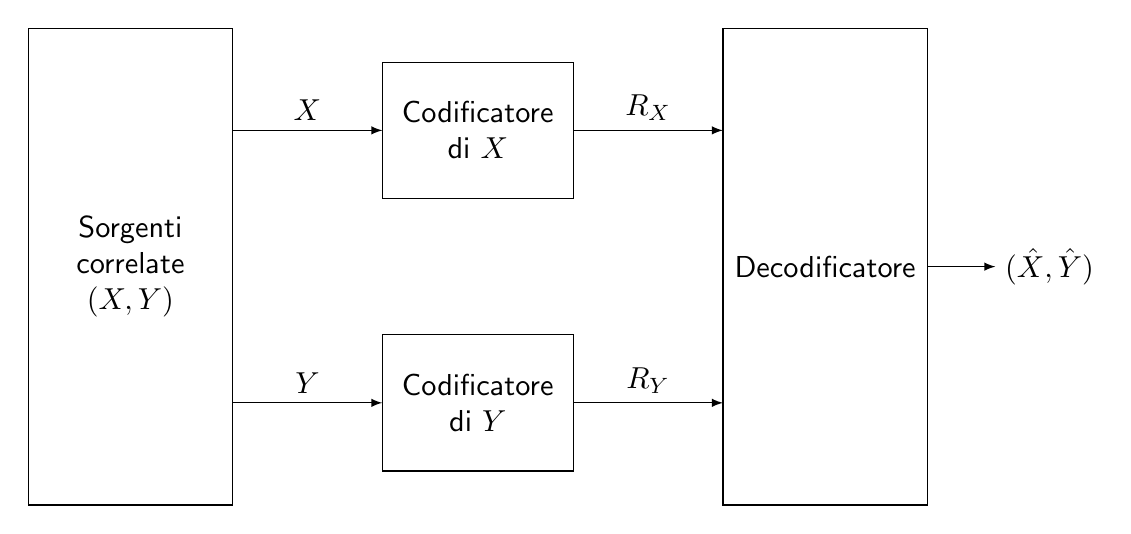
\begin{tikzpicture}[scale=0.865,>=latex]
    \tikzstyle{every node}=[font=\fontsize{11}{13}\sffamily]

    \draw (0,0) rectangle (3,7)
    node[midway,align=center]{Sorgenti \\ correlate \\ \((X,Y)\)};

    \draw[->] (3,5.5) -- (5.2,5.5)
    node[above,midway]{\(X\)};

    \draw[->] (3,1.5) -- (5.2,1.5)
    node[above,midway]{\(Y\)};

    \draw (5.2,4.5) rectangle (8,6.5)
    node[midway,align=center]{Codificatore \\ di \(X\)};

    \draw (5.2,0.5) rectangle (8,2.5)
    node[midway,align=center]{Codificatore \\ di \(Y\)};

    \draw[->] (8,5.5) -- (10.2,5.5)
    node[above,midway]{\(R_X\)};

    \draw[->] (8,1.5) -- (10.2,1.5)
    node[above,midway]{\(R_Y\)};

    \draw (10.2,0) rectangle (13.2,7)
    node[midway]{Decodificatore};

    \draw[->] (13.2,3.5) -- (14.2,3.5)
    node[right]{\((\hat{X},\hat{Y})\)};
\end{tikzpicture}

    \caption{Configurazione per la codifica di sorgente Slepian-Wolf.}
    \label{fig:sw-configuration}
\end{figure}

\begin{thm}[Slepian-Wolf \textnormal{\cite{10.1002/047174882X.ch15}}]
    \label{thm:sw}

    Sia \((X_1,Y_1),(X_2,Y_2),\dots\) una sequenza di variabili aleatorie
    congiunte, indipendenti e identicamente distribuite tali che la generica
    coppia \((X,Y) \sim p(x, y)\).\\
    Per il problema della codifica di sorgenti distribuite per la sorgente
    \((X,Y)\), la regione di tasso raggiungibile è data da
    \begin{alignat}{1}
        R_X &\ge \entropy{X \vert Y}, \label{eq:SW1} \\
        R_Y &\ge \entropy{Y \vert X}, \label{eq:SW2} \\
        R_X + R_Y &\ge \entropy{X,Y}. \label{eq:SWsum}
    \end{alignat}
\end{thm}

La Figura~\ref{fig:sw-rate-region} mostra la regione descritta dal
Teorema~\ref{thm:sw}.

\begin{figure}[ht]
    \centering
    \begin{tikzpicture}[>=latex]
    %\tikzstyle{every node}=[font=\fontsize{11}{13}\sffamily]

    \draw[->] (0,0) -- (8,0)
    node[right]{\(R_X\)};

    \draw[->] (0,0) -- (0,6)
    node[above]{\(R_Y\)};

    \draw (1.8,3pt) -- (1.8,-3pt)
    node[anchor=north]{\(\entropy{X \vert Y}\)};

    \draw (3.6,3pt) -- (3.6,-3pt)
    node[anchor=north]{\(\entropy{X}\)};

    \draw (7.2,3pt) -- (7.2,-3pt)
    node[anchor=north]{\(\entropy{X,Y}\)};

    \draw (3pt,2) -- (-3pt,2)
    node[anchor=east]{\(\entropy{Y \vert X}\)};

    \draw (3pt,3) -- (-3pt,3)
    node[anchor=east]{\(\entropy{Y}\)};

    \draw (3pt,4) -- (-3pt,4)
    node[anchor=east]{\(\entropy{X,Y}\)};

    \draw[help lines] (7.2,0) -- (0,4);
    \draw[help lines] (1.8,0) -- (1.8,5.5);
    \draw[help lines] (3.6,0) -- (3.6,2);
    \draw[help lines] (0,2) -- (7,2);
    \draw[help lines] (0,3) -- (1.8,3);

    \draw (3.6,2) -- (7,2);
    \draw (3.6,2) -- (1.8,3);
    \draw (1.8,5.5) -- (1.8,3);

    \foreach \x in {2.64,2.74,...,6}
    \draw[xslant=0.5] (\x cm,2) -- (\x cm,2.22);

    \foreach \x in {0.2,0.3,...,2.2}
    \draw[rotate=-29.055] (\x cm,3.5) -- (\x cm,3.75);

    \foreach \y in {-0.2,-0.04,...,2.22}
    \draw[yslant=1.8] (1.8,\y cm) -- (1.925,\y cm);

    \draw (4,3.5) node{\(\mathcal{R}\)};
\end{tikzpicture}

    \caption{Regione \(\mathcal{R}\) di tasso raggiungibile con la codifica di
    sorgente Slepian-Wolf.}
    \label{fig:sw-rate-region}
\end{figure}


\section{Approccio feedback-only}

Mostriamo adesso l'ottimalità dell'approccio feedback-only per la
segnalazione del CSI quando un tasso di segnalazione variabile viene
utilizzato. Per semplicità di derivazione, assumiamo che entrambi i canali
\(\bm{h}^\mathrm{(U)}\) e \(\bm{h}^\mathrm{(D)}\) possano essere rappresentati
da alfabeti di dimensione finita molto grande. In particolare, per
\(\bm{h}^\mathrm{(D)}\), consideriamo una quantizzazione tale da garantire
l'MSE desiderato sul canale di DL alla BS. Quindi, assumiamo che la BS intenda
ricostruire perfettamente il canale di DL senza distorsione. Inoltre, imponiamo
un vincolo solamente sul numero totale di bit della segnalazione \(B\), senza
ulteriormente richiedere un bilanciamento tra i tassi di segnalazione in UL e
DL.

\begin{thm}
    \label{thm:feedback-only}

    Per una procedura di segnalazione che utilizza un feedback a tasso
    variabile con media \(b_\mathrm{B}\) e un feedforward a tasso variabile con
    media \(b_\mathrm{F}\), il tasso minimo totale della segnalazione \(B =
    b_\mathrm{B} + b_\mathrm{F}\) è ottenuto con un approccio feedback-only,
    ovvero per \(b_\mathrm{F} = 0\).
\end{thm}

\begin{proof}
    Possiamo vedere la procedura di feedback come una codifica Slepian-Wolf
    (vedi Sezione~\ref{sec:correlated-sources-encoding}) nella quale le due
    sorgenti correlate (i canali di UL e DL) vengono codificate separatamente e
    poi inviate a una destinazione (la BS) che deve ricostruire entrambe. Si
    noti che nel nostro scenario il canale di UL è già noto alla BS, di
    conseguenza questa parte della codifica risulta banale. Ora, in presenza
    di feedforward, lo UT conosce sia la variabile di feedforward
    \(c^\mathrm{(F)}\) che rappresenta la versione quantizzata di
    \(\bm{h}^\mathrm{(U)}\) che il canale di DL \(\bm{h}^\mathrm{(D)}\).
    Pertanto, denotano con \(R_\mathrm{L}\) il tasso medio per la
    rappresentazione locale del canale di UL alla BS, il teorema di
    Slepian-Wolf fornisce
    \begin{alignat}{1}
        b_\mathrm{B} &\ge \entropy{
            \bm{h}^\mathrm{(D)},c^\mathrm{(F)} \given \bm{h}^\mathrm{(U)}
        }, \label{eq:fo-proof-1} \\
        R_\mathrm{L} &\ge \entropy{
            \bm{h}^\mathrm{(U)} \given \bm{h}^\mathrm{(D)},c^\mathrm{(F)}
        }, \label{eq:fo-proof-2} \\
        b_\mathrm{B} + R_\mathrm{L} &\ge \entropy{
            \bm{h}^\mathrm{(D)},\bm{h}^\mathrm{(U)},c^\mathrm{(F)}
        }. \label{eq:fo-proof-3}
    \end{alignat}
    Si noti che, dal momento che non ci sono limitazioni per la
    rappresentazione interna del canale di UL alla BS, la \eqref{eq:fo-proof-2}
    e la \eqref{eq:fo-proof-3} sono trascurabili, o in altre parole, non è
    limitante porre \(R_\mathrm{L} = \infty\); quindi, la sola condizione
    rilevante è
    \begin{equation}
        \label{eq:fo-proof-4}
        b_\mathrm{B} \ge \entropy{
            \bm{h}^\mathrm{(D)},c^\mathrm{(F)} \given \bm{h}^\mathrm{(U)}
        }.
    \end{equation}
    Tuttavia, poiché \(c^\mathrm{(F)}\) è funzione deterministica di
    \(\bm{h}^\mathrm{(U)}\), la \eqref{eq:fo-proof-4} risulta equivalente a
    \begin{equation}
        \label{eq:fo-proof-5}
        b_\mathrm{B} \ge \entropy{
            \bm{h}^\mathrm{(D)} \given \bm{h}^\mathrm{(U)}
        }.
    \end{equation}
    Quindi, abbiamo dimostrato che la segnalazione in feedforward non è utile
    al fine di ridurre i bit di feedback.
\end{proof}

Si noti come, considerando una codifica di sorgenti correlate distribuite
Slepian-Wolf, il risultato ottenuto corrisponde al caso in cui una delle due
sorgenti, anziché essere codificata e inviata al decodificatore, assume il
ruolo di informazione laterale. Infatti, una stima del canale di UL
\(\bm{h}^\mathrm{(U)}\) è già presente alla BS, e l'unica sorgente che
dev'essere codificata (dallo UT) e inviata al decodificatore (la BS) è il
canale di DL \(\bm{h}^\mathrm{(D)}\).

Inoltre, vogliamo sottolineare il fatto che questo risultato è valido in
assenza di condizioni che sbilanciano i tassi di segnalazione in UL e DL,
ovvero quando non ci sono ulteriori limitazioni su \(b_\mathrm{B}\) e
\(b_\mathrm{F}\). Nella pratica, gli svantaggi nel segnalare in UL e DL
potrebbero essere differenti, e soluzioni alternative potrebbero divenire
praticabili.


\section{Procedura di codifica}

\lipsum[4]

